\documentclass[letter]{ieicej}
\usepackage[dvipdfmx]{graphicx,xcolor}
\usepackage[fleqn]{amsmath}
\usepackage{newtxtext}
\usepackage[varg]{newtxmath}
\usepackage{url}
\makeatletter\def\hyper@nopatch@bib{}\makeatother
\usepackage[dvipdfmx,hidelinks]{hyperref}
\typeofletter{研究速報}
\field{}
\jtitle{LLMエージェントにおける履歴要約方式と\\終了制御の総トークン数評価}
\etitle{Evaluating Total Token Usage of History Summarization Methods and Termination Control for LLM Agents}
\authorlist{\authorentry{著者未設定}{Author details pending}{}{}\MembershipNumber{}}
\jalcdoi{???????????}
\clubpenalty=10000
\widowpenalty=10000
\raggedbottom
\begin{document}
\maketitle
\begin{abstract}
LLMエージェントの履歴要約方式とAPI実行記録に基づく終了制御を独立に評価する．要約生成を含む全モデル呼出しを計測し，既知課題の成功を保つ総トークン数の削減を確認した．呼出し配置と完了後の生成に着目した実行管理の比較結果を示す．
\end{abstract}
\begin{keyword}
LLMエージェント，ハーネス，履歴要約，終了制御，トークン使用量
\end{keyword}
\begin{eabstract}
We independently evaluated history summarization methods and termination control based on API execution records for LLM agents. Counting all model calls, including dedicated summarization, showed reductions in total tokens while preserving success on known tasks under the evaluated conditions.
\end{eabstract}
\begin{ekeyword}
LLM agents, harness, history summarization, termination control, token usage
\end{ekeyword}

% Single-column tables; scientific values unchanged from v08.
\newcommand{\SummaryResultsTable}{%
\begin{table}[!ht]
\caption{実験Aの課題別総トークン数}
\label{tab:summary}
\centering\fontsize{7}{9}\selectfont
\begin{tabular*}{65mm}{@{\extracolsep{\fill}}lrrr@{}}\hline
課題 & \shortstack{専用1回\\方式} & \shortstack{専用反復\\方式} & \shortstack{行動併記\\方式}\\\hline
写真操作 & 139,871 & 139,871 & 129,374\\
精算 & 211,110 & 211,110 & 211,110\\
返金 & 102,087 & 102,087 & 102,087\\
CSV処理 & 440,461 & 332,588 & 394,351\\\hline
合計 & 893,529 & 785,656 & 836,922\\\hline
\end{tabular*}
\end{table}}

\newcommand{\TerminationResultsTable}{%
\begin{table}[!ht]
\caption{実験Bの総トークン数と呼出し回数}
\label{tab:termination}
\centering\fontsize{7}{9}\selectfont
\begin{tabular*}{65mm}{@{\extracolsep{\fill}}llrrr@{}}\hline
API条件 & 終了方法 & 総トークン数 & \shortstack{モデル\\呼出し数} & \shortstack{API\\要求数}\\\hline
文書必須 & 通常継続 & 130,439 & 15 & 104\\
文書必須 & 終了制御 & 91,116 & 13 & 100\\[2pt]
名前参照 & 通常継続 & 151,664 & 14 & 103\\
名前参照 & 終了制御 & 112,233 & 12 & 99\\\hline
\end{tabular*}
\end{table}}


\section{はじめに}

日常業務のデータ整理や事務処理の負担を軽減するため，大規模言語モデルによる作業支援が研究されている．以下では大規模言語モデルをLLMと呼ぶ．文章の回答生成に加え，外部アプリケーションを操作する複数手順の実行も対象となる．例えば写真の整理や精算では，対象の検索，状態の変更，結果の確認を連続して行う必要がある．推論と行動を繰り返すReAct\cite{yao2023react}や，コードを行動として実行するCodeAct\cite{wang2024codeact}は，このような対話的処理を支える技術である．

一方，実行が長くなると，過去の操作と観測を次の生成へ繰り返し入力する費用が増える．また，作業が終わった後も確認や生成を続ければ，成果を増やさずに資源を消費し得る．履歴を短くするだけでは必要な情報を失うおそれがあり，早く止めるだけでは未完了となり得るため，最終成功と実行全体の費用を同時に調べる必要がある．

本稿では，モデルを再学習せずに実行を管理するハーネスについて，履歴要約の呼出し配置と終了制御を評価する．履歴要約では，要約を生成する時点，行動生成と呼出しを分けるかどうか，要約機会の上限を比較軸とする．終了制御では，実行中に取得できるAPIの要求と応答を記録し，このAPI実行記録に基づく制御を通常継続と比較する．両者を独立した実験として実行し，要約生成を含む全モデル呼出しの総トークン数と，課題の最終成功を調べる．

\par\noindent\begin{minipage}{\columnwidth}
\section{関連研究}

入力圧縮では，長文中の情報の位置が性能に影響すること\cite{liu2024lost}を踏まえ，LLMLingua\cite{jiang2023llmlingua}は予算制御とトークン選別，LLMLingua-2\cite{pan2024llmlingua2}は蒸留データによるトークン分類，LongLLMLingua\cite{jiang2024longllmlingua}は長文の重要情報を残す圧縮を扱う．

\end{minipage}\par\penalty0

長期実行では，ACON\cite{kang2026acon}は観測・履歴の圧縮方針，TokenPilot\cite{xu2026tokenpilot}は入力圧縮とキャッシュ継続性を扱う．Generative Agents\cite{park2023generative}は経験の記憶・抽象化・検索，Reflexion\cite{shinn2023reflexion}は言語的フィードバックを後続試行に利用する．本稿は，要約を専用の呼出しで生成する方式と，行動と同じ応答に含める方式を比べ，要約生成も含む課題全体のトークン使用量を評価する．

終了制御では，Runaway\cite{lu2025runaway}が終了指示と外部の完了検証を検討している．本稿では，既知の要求形式についてAPI実行記録から完了条件を検査する．通常継続との比較では，最終成功，API要求数，総トークン数を評価する．

\section{提案手法}

ハーネスは，モデルの外側で入力と実行の継続を管理するプログラムである．本稿では，既存の要約を使って入力履歴を更新する処理と，API実行記録を使って次の生成の要否を判断する処理を構成する．図\ref{fig:architecture}の実験Aには要約と行動生成の呼出し配置を，実験Bには完了判定に基づく終了制御を示す．両者は別々に評価し，組合せによる削減は扱わない．

\subsection{入力履歴を短くする制御}

まず，課題とこれまでの履歴をモデルへ渡し，次に実行する行動を生成する．ハーネスは生成されたプログラムを実行し，その行動と結果を履歴に追加する．行動生成から実行結果の記録までを1ターンとする．

\begin{figure*}[!t]
\centering
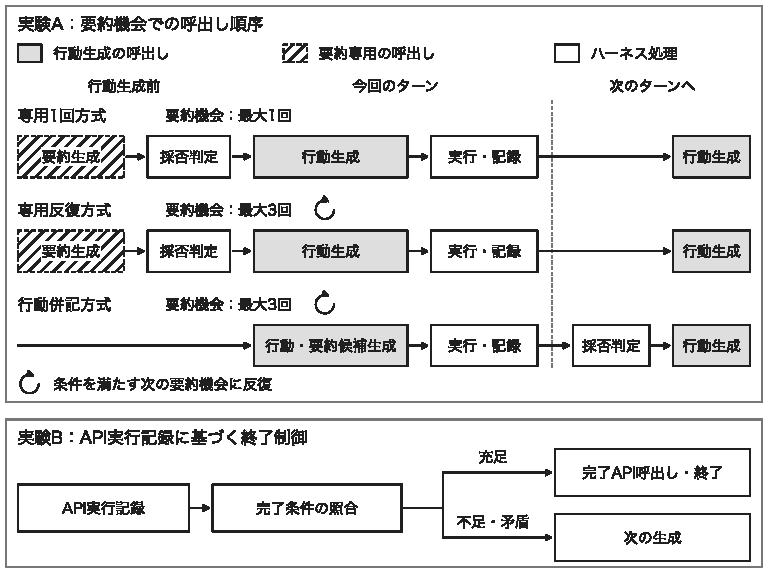
\includegraphics[width=130mm]{figures/control_points.pdf}
\capwidth=130mm\ecapwidth=130mm
\abovecaptionskip=1pt\belowcaptionskip=1pt
\caption{履歴要約方式と終了制御}
\label{fig:architecture}
\end{figure*}

この繰返しで長くなる入力を抑えるため，保存した全履歴は残したまま，モデルへ渡す古い履歴を要約に置き換える．生成した要約を，検査して採用する前は要約候補と呼ぶ．本稿では，要約を生成するためだけに行うモデル呼出しを専用呼出しとし，次の3方式に比較用の名称を付ける．

専用1回方式は，要約専用のモデル呼出しを最大1回追加する方式である．入力長が閾値に達し，要約できる古い履歴がある最初の要約機会に候補を生成する．候補を検査し，採用する場合は要約と未要約の履歴を次の行動生成へ渡す．要約機会は最大1回とし，その機会の終了後は新たな要約機会を設けない．

専用反復方式は，要約専用の呼出しを必要に応じて繰り返す方式である．最初の要約機会では，専用1回方式と同じ処理を行う．以後，入力長と新たに完了したターン数の条件を満たすと，その時点で未要約の古い履歴を要約対象とする．採用済みの要約がある場合は，その要約も対象に含める．要約機会は最大3回とし，各機会で候補の採否を決めてから次の行動を生成する．

行動併記方式は，行動を生成するモデルの同じ応答に，行動と要約候補を出力する方式である．要約専用の呼出しは追加せず，最大3回の要約機会を設ける．この応答内の全プログラムを実行し，結果を記録してから，次の行動生成へ進む前に候補の採否を決める．候補には，その応答で生成した行動の実行結果は含めない．その行動と実際の結果は原文のまま次の入力に残す．

どの方式でも，要約には完了した作業，次の操作に使う情報，残作業，不確かな点の四つの欄を用いる．候補が得られたら，ハーネスが形式と文字数を検査する．さらに，元の指示と課題，要約，未要約の履歴を含む次回入力全体のトークン数を比べ，候補を採用しない場合より厳密に少なくなることを確認して採用する．要約候補を生成する時点で，直近2ターンを原文のまま残す．検査するのは構造と入力長であり，要約内容の正しさを保証するものではない．

完了した作業の欄には実行済みの内容を，次の操作に使う情報の欄には識別子，APIの呼出し方，保持された変数などを残すよう指示する．残作業と不確かな点の欄では，未実施の操作と未確認の事項を区別する．APIの正常応答だけから課題の完了を推定しないよう求める．

元の指示と課題は要求の基準として残し，直近の行動とAPI応答も原文で渡す．これにより，古い履歴の提示方法を変えながら，要求と直近の実行結果を参照できる構成とする．

採用条件を満たさなければ，それまでの要約と未要約の履歴を維持する．まだ要約を採用していない場合は，要約前の履歴を使い続ける．要約機会は候補の生成を試みる機会であり，採用回数とは区別する．不採用の場合も1回の機会として数え，その場で候補の再生成は行わない．専用1回方式は機会の上限を定める名称であり，生成や採用が0回となる場合もある．入力長とターン数の閾値は4.1に示す．保存した全履歴は，入力を短くした後も別に残す．

専用呼出しでは候補の生成に1回のモデル呼出しを使うが，行動併記方式では行動生成の呼出しを共有する．一方，採用回数は入力を実際に更新した回数である．本稿では要約機会数，採用回数，モデル呼出し数を明確に区別して扱う．採用後も新しい行動と結果は未要約の履歴として追加され，次の要約機会まで入力に残る．

\subsection{作業完了後の生成を省く制御}

終了制御は，API実行記録から課題の完了を検査し，根拠が揃った時点で次の生成を省く処理である．この検査の段階を完了判定と呼ぶ．写真を作成時期に応じた指定先へ移す課題を対象とし，既知の一つの要求形式に対応する検査規則を手書きで用意する．まず，モデル応答内の全プログラムを実行し，APIの要求と応答を記録する．次に，移動前の写真一覧と各写真の作成日時，APIから取得した現在年を確認する．これらに基づいて，全ての対象が指定先へ移され，元の名前が保たれているか照合する．完了の根拠が初めて揃った時点で完了APIを1回呼び出し，次の生成を省く．

完了判定は，モデルの完了宣言ではなく，API実行記録に対象全件の処理を確認できる情報があるかを調べる．通常継続は，この判定による終了を行わず，通常の実行手順を続ける比較条件である．

対象集合を移動前に確定するのは，一部の移動だけで完了と判断することを避けるためである．作成日時とAPIから得た現在年は，写真ごとに指定された移動先を照合する際に使う．移動後の場所に加えて元の名前の保持を調べることで，指定先へ移すという要求と，名前を変えないという要求を別々に確認する．これらの根拠はモデルの推測や計算機の時刻で補わず，API実行記録から取得する．

対応する要求形式から外れる場合や，判定に必要な記録が不足・矛盾する場合は，通常どおり次の生成へ進む．判定には，その時点で得られたAPI実行記録だけを使い，公式評価器の正解は使わない．履歴要約との組合せ効果は評価しない．

\subsection{総トークン数と課題の成功}

1回の入力を短くしても，要約生成やその後の行動生成に使用するトークンが増えれば，課題全体の使用量は増え得る．そこで，要約後の入力だけを比べず，課題開始から終了までを全方式に共通する集計範囲とする．

\par\noindent\begin{minipage}{\columnwidth}
\setlength{\abovedisplayskip}{4pt}\setlength{\belowdisplayskip}{4pt}
条件$p$で実行したモデル呼出しの集合を$\mathcal C_p$とする．各呼出し$c$の入力トークン数を$I_c$，出力トークン数を$O_c$とし，実行全体の総トークン数$T_p$を\mbox{式\eqref{eq:cost}で求める．}

\begin{equation}
 T_p=\sum_{c\in\mathcal C_p}(I_c+O_c)
 \label{eq:cost}
\end{equation}

要約にも生成費用がかかるため，行動生成と要約生成の両方を集計する．不採用となった要約の生成や失敗時の呼出しも，取得できた使用量を計上する．使用量が不明な場合は0とせず，既知分の小計と不明件数を記録する．

\end{minipage}\par\penalty0

課題の成功は，実行終了後の状態に対するAppWorld\cite{trivedi2024appworld}の公式評価器で判定する．評価器の正解や詳細は実行中のモデルへ返さない．方式間では成功数と，各課題の成功の維持を確認する．

同じ課題を処理した方式同士で成功と総トークン数を対応させる．課題をまたぐ合計では減少と増加が相殺されるため，実験Aでは課題別の値も示す．

本指標はキャッシュされた入力も含む論理トークン数であり，金銭課金や実行時間を直接表すものではない\cite{xu2026tokenpilot}．要約生成を含む費用評価はACON\cite{kang2026acon}にも用いられている．実験AとBは独立に集計する．履歴要約は次回入力の長さ，終了制御は次の生成の必要性を管理する．判断に使う材料と変更する対象が異なるため，それぞれの制御と対照を独立に比較する．

\section{実験A：要約の呼出し配置}

\subsection{条件}

写真操作，精算，返金，CSV処理の既知4課題に対し，専用1回方式，専用反復方式，行動併記方式の各方式を各課題で1回ずつ実行した．4課題に3方式を適用し，計12実行とした．モデルは全条件でMiniMax-M3を用い，GGUF形式のIQ4\_XS量子化モデルをllama.cpp b11669で実行した．文脈長は65,536トークンである．乱数の初期値を表すseedは，モデル生成の基点を57，環境を42とした．生成側は呼出しの役割と順序に従いseedを増分した．

要約機会を設ける入力長の閾値は16,384トークンとし，要約時には直近2ターンを原文のまま保持する．専用反復方式と行動併記方式では，前回の要約機会が終了してから新たに3ターン以上が完了することを要求する．採用と不採用のどちらでも，その機会の終了時点を次回の起点とする．初回の起点は課題開始である．要約は合計8,192文字以下とし，次の行動生成へ渡す入力全体が短くなる場合に採用する．要約専用の呼出しでは出力上限を4,096トークンとし，その使用量も式\eqref{eq:cost}へ含める．

各実行の上限はモデル呼出し80回，総トークン数450,000，作業時間1,800秒とし，環境APIは写真160，他3課題80要求とした．生成の温度は行動生成で1.0，要約専用の生成で0.7とした．並列実行数は1，KVキャッシュはq8\_0，計算機はApple M3 Ultra，メモリは256 GiBである．実装と記録を公開する\footnote{\url{https://github.com/sophiria1225/AI-}}．

\subsection{全4課題の結果}

表\ref{tab:summary}に4課題の結果を示す．全12実行で課題に成功し，使用量の欠測はなかった．

\SummaryResultsTable

要約生成を含む4課題の合計は，専用反復方式が785,656トークンで3方式中最少だった．専用1回方式の893,529トークンに対し107,873トークン少なく，削減率は12.07\%だった．この差はCSV処理だけで生じ，残る3課題では両方式の値が一致した．

写真操作では，専用1回方式と専用反復方式は139,871トークンで，行動併記方式は129,374トークンだった．行動併記方式は他の2方式より10,497トークン少なかった．要約の採用回数はいずれも1回だった．同じ1回の要約採用でも，課題全体の総トークン数には差があった．

精算の総トークン数は全方式で211,110トークンだった．いずれも要約の採用回数は0回で，方式による総量の差はなかった．

返金では，全方式で102,087トークンを使用し，要約の採用回数は0回だった．精算と同様に，成功と総トークン数は全方式で一致した．

CSV処理では，専用1回方式は440,461，専用反復方式は332,588，行動併記方式は394,351トークンだった．専用反復方式は専用1回方式より107,873トークン少なく，4課題合計の削減はこの課題で生じた．要約の採用回数は専用1回方式が1回，専用反復方式と行動併記方式が各2回だった．専用反復方式と行動併記方式の採用回数は等しかったが，総トークン数は一致しなかった．

行動併記方式は4課題合計で専用1回方式より6.34\%少なかったが，専用反復方式より51,266トークン多く，増加率は6.53\%だった．専用反復方式との比較では，写真操作で10,497トークン減る一方，CSV処理で61,763トークン増えた．要約専用の呼出しを省く構成でも，課題全体の総トークン数が最少になるとは限らなかった．表\ref{tab:summary}の課題別の値と合計を併記することで，異なる課題で生じた減少と増加を分けて確認できる．

\section{実験B：API実行記録に基づく終了制御}

\subsection{条件}

同じ写真課題について，API文書の取得を必須とする文書必須条件と，公開API名からのアクセスを許す名前参照条件を設けた．各条件で，通常継続と，API実行記録に基づく終了制御を比較した．終了制御は，事前に実行・保存した通常継続と同じ初期状態，モデル，seed，モデルへの指示とツール説明，予算を用いて各1回実行した．

seedの基点は42であり，実験Aとは別の履歴・設定である．同じMiniMax-M3 IQ4\_XSとllama.cpp b11669を用い，各実行の予算はモデル呼出し80回，450,000トークン，1,800秒，API160要求とした．

完了判定と完了通知は3.2に従う．判定，記録保存，完了通知を含む実行時間を記録し，完了通知をAPI要求数に含めた．

行動の生成はLLMが担い，記録の検査はハーネスの規則で行う．この検査のために別のモデル呼出しは設けない．完了の根拠が揃えば次の行動生成を省き，根拠が足りなければ同じ実行を継続する．

終了以前の生成過程の違いが比較に含まれていないか確認するため，終了制御側で実行したモデル呼出しの要求と応答が，通常継続側の先頭から同じ範囲と完全に一致することを事前の照合基準とした．API操作の記録と最終状態も比較した．

\subsection{成功を保った総トークン数の削減}

表\ref{tab:termination}に結果を示す．両API条件で課題の成功を保ち，終了制御により総トークン数を削減した．文書必須では130,439から91,116へ30.15\%，名前参照では151,664から112,233へ26.00\%減った．全4実行で公式評価器による成功を確認し，使用量の欠測はなかった．各条件でモデル呼出し2回とAPI要求4回を削減した．完了通知を含めて処理を終え，移動後の4回の確認APIと，それに伴う生成を省いた．

\TerminationResultsTable

\par\noindent\begin{minipage}{\columnwidth}
実行したAPI操作などの前半の記録と，実行終了時の13個のデータベースのハッシュ値は対照と一致し，最終状態を保った削減を確認した．一方，要求・モデル応答全文の完全一致基準は満たさなかった．このため，観測した差の全てを終了制御のみの効果とは断定せず，既知の要求形式に対する各1回の比較として扱う．平均的な因果効果や汎用的な終了保証を示す評価ではない．
\end{minipage}\par\penalty0

\section{むすび}

既知4課題全てで成功を保ち，専用反復方式の総トークン数は専用1回方式を12.07\%下回った．この差はCSV処理によるものであり，他3課題の値は一致する．行動併記方式の合計は専用反復方式より6.53\%多い．独立に評価した写真課題の2つのAPI条件では，終了制御を用いた実行で成功を保ち，通常継続に比べて26.00--30.15\%の削減を確認した．本評価は，要約生成を含む全モデル呼出しの計測と，API実行記録から得られる完了の根拠に基づく実行管理の意義を示す．

本稿は，既知課題と単一モデル・量子化設定における少数のseed・試行による開発実験を事後に整理した評価である．未見課題の品質維持や統計的非劣性は評価していない．

% Twelve formal conference/journal papers. Source verification: reference_update.json.
\begin{thebibliography}{99}
\bibitem{yao2023react}
S. Yao, J. Zhao, D. Yu, N. Du, I. Shafran, K. Narasimhan, and Y. Cao,
``ReAct: Synergizing reasoning and acting in language models,''
Proc. ICLR, May 2023.

\bibitem{wang2024codeact}
X. Wang, Y. Chen, L. Yuan, Y. Zhang, Y. Li, H. Peng, and H. Ji,
``Executable code actions elicit better LLM agents,''
Proc. ICML, PMLR, vol.235, pp.50208--50232, July 2024.

\bibitem{liu2024lost}
N. F. Liu, K. Lin, J. Hewitt, A. Paranjape, M. Bevilacqua, F. Petroni, and P. Liang,
``Lost in the middle: How language models use long contexts,''
Trans. ACL, vol.12, pp.157--173, 2024.
doi: 10.1162/tacl\_a\_00638.

\bibitem{jiang2023llmlingua}
H. Jiang, Q. Wu, C.-Y. Lin, Y. Yang, and L. Qiu,
``LLMLingua: Compressing prompts for accelerated inference of large language models,''
Proc. EMNLP, pp.13358--13376, Dec. 2023.
doi: 10.18653/v1/2023.emnlp-main.825.

\bibitem{pan2024llmlingua2}
Z. Pan, Q. Wu, H. Jiang, M. Xia, X. Luo, J. Zhang, Q. Lin, V. R\"uhle,
Y. Yang, C.-Y. Lin, H. V. Zhao, L. Qiu, and D. Zhang,
``LLMLingua-2: Data distillation for efficient and faithful task-agnostic prompt compression,''
Findings of ACL: ACL 2024, pp.963--981, Aug. 2024.
doi: 10.18653/v1/2024.findings-acl.57.

\bibitem{jiang2024longllmlingua}
H. Jiang, Q. Wu, X. Luo, D. Li, C.-Y. Lin, Y. Yang, and L. Qiu,
``LongLLMLingua: Accelerating and enhancing LLMs in long context scenarios via prompt compression,''
Proc. ACL, vol.1, pp.1658--1677, Aug. 2024.
doi: 10.18653/v1/2024.acl-long.91.

\bibitem{kang2026acon}
M. Kang, W.-N. Chen, D. Han, H. A. Inan, L. Wutschitz, Y. Chen,
R. Sim, and S. Rajmohan,
``ACON: Optimizing context compression for long-horizon LLM agents,''
Proc. ICML, PMLR, vol.306, pp.55321--55375, July 2026.

\bibitem{xu2026tokenpilot}
B. Xu, Z. Xue, D. Chen, C. Fu, C. Wu, C. Huang, C. Jiang, J. Fang,
X. Deng, Y. Chen, Y. Yao, X. Wang, J. Shang, H. Chen, and N. Zhang,
``TokenPilot: Cache-efficient context management for LLM agents,''
Findings of ACL: EMNLP 2026, pp.19034--19049, Oct. 2026.

\bibitem{park2023generative}
J. S. Park, J. O'Brien, C. J. Cai, M. R. Morris, P. Liang, and M. S. Bernstein,
``Generative agents: Interactive simulacra of human behavior,''
Proc. ACM UIST, article 2, pp.1--22, Oct. 2023.
doi: 10.1145/3586183.3606763.

\bibitem{shinn2023reflexion}
N. Shinn, F. Cassano, A. Gopinath, K. Narasimhan, and S. Yao,
``Reflexion: Language agents with verbal reinforcement learning,''
Advances in Neural Information Processing Systems, vol.36, pp.8634--8652, 2023.
doi: 10.52202/075280-0377.

\bibitem{lu2025runaway}
Q. Lu, L. Ding, S. Cao, X. Liu, K. Zhang, J. Zhang, and D. Tao,
``Runaway is ashamed, but helpful: On the early-exit behavior of large language model-based agents in embodied environments,''
Findings of ACL: EMNLP 2025, pp.24014--24027, Nov. 2025.
doi: 10.18653/v1/2025.findings-emnlp.1304.

\bibitem{trivedi2024appworld}
H. Trivedi, T. Khot, M. Hartmann, R. Manku, V. Dong, E. Li, S. Gupta,
A. Sabharwal, and N. Balasubramanian,
``AppWorld: A controllable world of apps and people for benchmarking interactive coding agents,''
Proc. ACL, vol.1, pp.16022--16076, Aug. 2024.
doi: 10.18653/v1/2024.acl-long.850.

\end{thebibliography}

\end{document}
